%Pakete;
%A4, Report, 12pt
\documentclass[ngerman,a4paper,12pt]{scrreprt}
\usepackage[a4paper, right=20mm, left=20mm,top=20mm, bottom=30mm, marginparsep=5mm, marginparwidth=5mm, headheight=7mm, headsep=15mm,footskip=15mm]{geometry}

%Papierausrichtungen
\usepackage{pdflscape}
\usepackage{lscape}

%Deutsche Umlaute, Schriftart, Deutsche Bezeichnungen
\usepackage[utf8]{inputenc}
\usepackage[T1]{fontenc}
\usepackage[ngerman]{babel}

%quellcode
\usepackage{listings}

%tabellen
\usepackage{tabularx}

%listen und aufzählungen
\usepackage{paralist}

%farben
\usepackage[svgnames,table,hyperref]{xcolor}

%symbole
\usepackage{latexsym,textcomp}

%font
\usepackage{helvet}
\renewcommand{\familydefault}{\sfdefault}

%Abkürzungsverzeichnisse
\usepackage[printonlyused]{acronym}

%Bilder
\usepackage{graphicx} %Bilder
\usepackage{float}	  %"Floating" Objects, Bilder, Tabellen...
\usepackage[space]{grffile} %Leerzechen Problem bei includegraphics
\usepackage{wallpaper} %Seitenhintergrund setzen
\usepackage{transparent} %Transparenz

%for
\usepackage{forloop}
\usepackage{ifthen}

%Dokumenteigenschaften
\title{Repetitionsfragen CN1}
\author{Tobias Blaser}
\date{\today{}, Rapperswil}


%Kopf- /Fusszeile
\usepackage{fancyhdr}
\usepackage{lastpage}

\pagestyle{fancy}
	\fancyhf{} %alle Kopf- und Fußzeilenfelder bereinigen
	\renewcommand{\headrulewidth}{0pt} %obere Trennlinie
	\fancyfoot[L]{Seite \thepage/\pageref{LastPage}} %Fusszeile mitte
	\fancyfoot[R]{\today{}} %Fusszeile rechts
	\renewcommand{\footrulewidth}{0.4pt} %untere Trennlinie

%Kopf-/ Fusszeile auf chapter page
\fancypagestyle{plain} {
	\fancyhf{} %alle Kopf- und Fußzeilenfelder bereinigen
	\renewcommand{\headrulewidth}{0pt} %obere Trennlinie
	\fancyfoot[L]{Seite \thepage/\pageref{LastPage}} %Fusszeile mitte
	\fancyfoot[R]{\today{}} %Fusszeile rechts
	\renewcommand{\footrulewidth}{0.4pt} %untere Trennlinie
}

\usepackage{changepage}

\input{../shortcuts}

%links, verlinktes Inhaltsverzeichnis, PDF Inhaltsverzeichnis
\usepackage[bookmarks=true,
bookmarksopen=true,
bookmarksnumbered=true,
breaklinks=true,
colorlinks=true,
linkcolor=black,
anchorcolor=black,
citecolor=black,
filecolor=black,
menucolor=black,
pagecolor=black,
urlcolor=black
]{hyperref} % Paket muss unbedingt als letzes eingebunden werden!

\usepackage{graphicx}
\begin{document}

% Inhaltsverzeichnis
\tableofcontents
\clearpage

\ch{Informationssysteme}
\ol
	\li Abb \ref{caseStudyFramework}: Erklären das  Case Study Framework
 	\begin{figure}[htp]
		\centering
		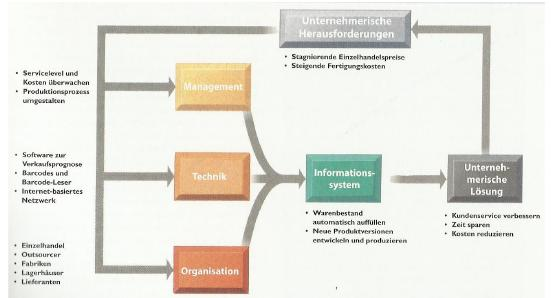
\includegraphics[scale=0.60]{img/R1.1.jpg}
		\caption{}
		\label{caseStudyFramework}
	\end{figure}
	\li Erklären Sie, was ein Informationssystem ist.
	\li Welchen Nutzen bringen Informationsysteme Firmen? Zählen sie vier punkte auf. 		\li Berücksichtigen Sie in einem zweiten Schritt vor allem die Vorteile in Bezug auf den Wettbewerb, in dem das Unternehmen steht.
	\li Welche vier gravierenden Veränderungen bringen Informationssysteme? Zählen Sie zu jeder einige Punkte auf, wie die Änderung konkret stattfindet / sich auswirkt.
	\li Wie verhalten sich „Digital Economy“ und „Economy of Scale“ in Bezug auf Stückkosten in Abhängigkeit der Ausbringungsmenge und Individualisierung in Abhängigkeit der Ausbringungsmenge. Warum?
	\li Definieren Sie, was ein IT-vernetztes Unternehmen ist und wie es entsteht.
\olS


\ch{Geschäftsprozesse}
\olR
	\li Was ist ein Geschäftsprozess?
	\li Was sind Daten, was ist Information?, Wie hängen Sie zusammen?
	\li Was ist ein Anwendungssystem und was ist ein Informationssystem? Wo ist der Zusammenhang?
	\li Welche Aufgaben übernimmt die Organisation in einem Unternehmen war?
	\li Was ist ein Wissensarbeiter? Was ein Datenverarbeiter?
	\li Welche Aufgabe übernehmen Top-, Middle- und Operative Management?
	\li Was sind ergänzende, organisatorische , managementbezogene und soziale Vermögenswerte?
	\li Was sind E-commerce und E-business? Was ist ein digitaler Markt? Was st E-Gouvernment?
	\li Welche sechs wichtigen Managementfragen sollten Sie sich stellen beim Aufbau und Einsatz von Informationsmanagementsystemen in Firmen?
\olS


\ch{Wirtschaft}
\olR
	\li In welchen Bereichen sind Betriebswirtschaft und Wirtschaftsinformatk anzusiedeln? Was bedeutet wirtschaften?
	\li Was sind Wirtschaftseinheiten? Nennen Sie drei.
	\li Ziele: Was sind Komplementärziele, konkurrierende Ziele und Indifferente Ziele?
	\li Zeichnen Sie den offenen Wirtschaftskreislauf inkl. Staat und Ausland.
	\li Was ist das St. Galler Management Modell und wie funktioniert es?
	\li Welche Gesellschafts- und Rechtsformen gibt es?
	\li Was ein Markt? Was sind Marktsegmentierung, Marktpotential, Marktvolumen, Marktanteil und Sättigungsgrad?
	\li Abb \ref{marktformen}: Erklären Sie die Marktformen und machen Sie Beispiele:
 	\begin{figure}[htp]
		\centering
		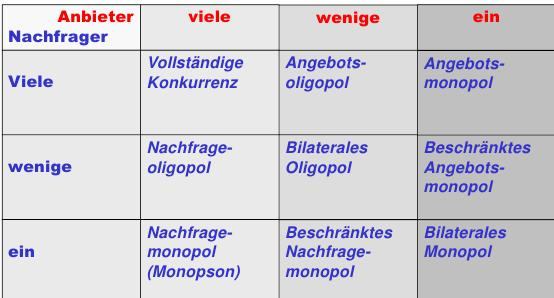
\includegraphics[scale=0.60]{img/R3.1.jpg}
		\caption{}
		\label{marktformen}
	\end{figure}
	\li Abb \ref{preisabsatzfunktion}: Erklären Sie die Preis-Absatzfunktion in Abhänigkeit der Marktnachfrage:
 	\begin{figure}[htp]
		\centering
		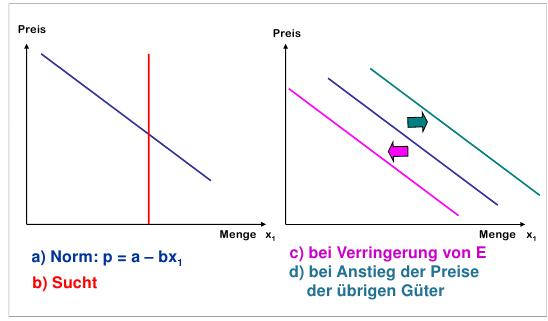
\includegraphics[scale=0.60]{img/R3.2.jpg}
		\caption{}
		\label{preisabsatzfunktion}
	\end{figure}
	\li Wie hängen Preis-Absatz und Umsatzerlös zusammen? Wie berechnen Sie den maximalen Umsatzerlös?
	\li Was ist die Preiselastizität dr Nachfrage? Welche Fälle liegen vor, wenn e < -1, e = 1 und -1 < e < 0? Was sind anomale Preiselastizitäten und welche gibt es?
	\li Wie hängen Unternehmensangebot und Preisangebot zusammen?
	\li Abb \ref{gewinnschwelle}: Erklären Sie folgende Grafik. Was passiert bei einer Preiserhöhung? Was bei einer Preisminderung?
 	\begin{figure}[htp]
		\centering
		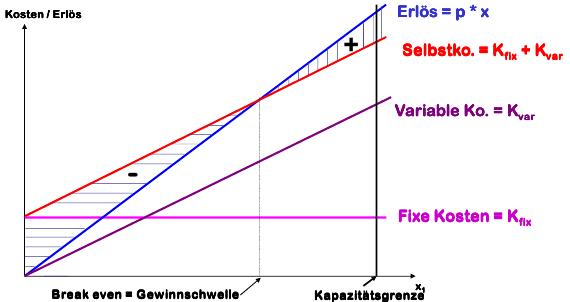
\includegraphics[scale=0.60]{img/R3.3.jpg}
		\caption{}
		\label{gewinnschwelle}
	\end{figure}
	\li Wie bildet sich der Marktpreis?
	\li Was ist das Spinnweb Theorem und was ist der Schweinezyklus?
	\li Wie ermitteln Sie die optimale Losgrösse?
\olS


\ch{Operative Anwendungssysteme}
\olR
	\li Was sind Anwendungssysteme? Unterscheiden Sie operative und Analytische AWS.
	\li Was unterscheidet Standard- und Individualsysteme? Nennen Sie je mindestens 6 Vor- oder Nachteile.s
	\li Was unterscheidet Büroinformations- und Vorgangsunterstützungssysteme?
	\li Was sind Workflowmanagementsysteme, Dokumentenmanagementsysteme, Wissensmanagementsysteme, Konferenzsysteme?
	\li Was sind Gemeinsame Arbeitsräume?
	\li Erklären Sie die Ein- und Ausgangskanäle eines DMS und erklären Sie die Möglichkeiten eines DMS.
	\li Wie funktionieren Wissensmanagementsysteme?
\olS

\ch{Operative Anwendungssysteme Forsetzung}
\olR
	\li Welche Ziele verfolgen Wissensmanagementsysteme und Wikis?
	\li Was bedeutet BestBride und was ist der Unterschied zu einem Gesammtsystem? Vor- / Nachteile?
	\li Wie ist eine Finanzbuchhaltung aufgebaut? Welche Komponenten übernehmen welche Aufgaben?
	\li Erklären Sie Branchenspezifische Software am Beispiel Produktionsplanungssystem und anhand eines Beispiels der Versicherungsbranche.
	\li Erklären Sie die Netzplantechnik.
\olS


\ch{Analytische Anwendungssysteme}
\olR
	\li Erklären Sie, was operative und analytische AWS unterscheidet.
	\li Abb. \ref{archAnaAWA}: Erklären Sie folgende Grafik:
	 	\begin{figure}[htp]
			\centering
			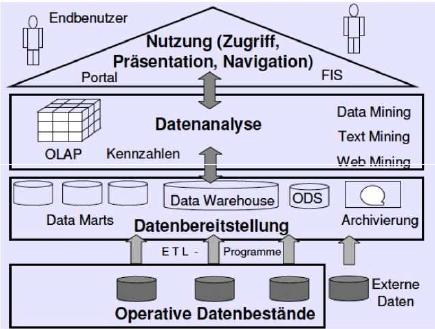
\includegraphics[scale=1]{img/R6.1.jpg}
			\caption{Architektur analytischer AWS}
			\label{archAnaAWA}
		\end{figure}
	\li Was ist ein Data Warehouse? Wozu wird es verwendet und Welche drei Arten von Architektur gibt es?
	\li  Erklären Sie den Unterschied zwischen Data Warehouse und Data Mart
	\li Was sind ETL Programme?
	\li Nennen Sie einige Mängel, die bei der Datenübernahme auftreten können. Was für Harmonisierungen können/müssen Sie durchführen?
	\li Was bedeutet eine Verdichtung, bezogen auf Analytische Daten?
	\li Was versteht man unter einem wöchtenlichen Ladeprozess in Bezug auf ETL Software?
	\li Welchen Mehrwert bieten Metadaten dem Benutzer?
	\li Stellen Sie "Operatives System", "ODS" und "Data Warehouse" einander gegenüber.
	\li Wie ist ein Data Warehouse aufgebaut.
	\li Erklären Sie den Unterschied zwischen Operativem IT-System und einem Data Warehouse.
	\li Was ist OLAP?
	\li Was ist mehrdimensionale Datenanalyse? Erklären Sie die folgenden Begriffe: Ad-Hoc-Sicht (Dice), Produktmanagersicht (SLice), Gebietsleitersicht(Slice), Controllersicht(Slice). Erklären Sie auch die verschiedenen Ansichten.
	\li Welche Navigationsmöglichkeiten haben Sie in einem OLAP Würfel?
	\li Erklären Sie folgende Datenstrukturen: Star-Schema, Snowflake-Schema, Multidimensionale Datenstruktur
	\li Was ist Data Mining.
	\li Erklären Sie den Datenanalyse-Zyklus von Data Mining.
	\li Erklären Sie den Data Mining Prozess.
	\li Erklären Sie die Unterschiede zwischen Data Mining, Text Mining und Web Mining.
	\li Was ist ein Data Mining Entscheidungsbaum?
	\li Was ist eine Assoziationsanalyse.
	\li Welche Diagrammform ist für welche Daten geeignet? Setzen Sie Kreuze: \newline
	\begin{tabular}{l|l|l|l|l|l|}
	& Kreis (k) & Balken (b) & Säule (s) & Kurve (ku) & Punkt (o) \\
	\hline
	Struktur (st) & & & & & \\
	\hline
	Rangfolge (r) & & & & & \\
	\hline
	Zeitreihe (z) & & & & & \\
	\hline
	Häufigkeit (h) & & & & & \\
	\hline
	Korrelation (ko) & & & & & \\
	\hline
	\end{tabular}
	\newline \newline
	Lösung: st: k, r: b s, z: s ku, h: s ku, ko: ku p
	\li Erklären Sie die folgenden Darstellungsmetaphern: Landkarten-Metapher, Organigramm-Metapher, Zeitungs-Metapher, Leitstand-Metapher
	\li Nennen Sie fünf Managementaktivitäten und die zugehörige Software-Funktion
	\li Was ist Exception Reporting? Wie wird es haufig visualisiert?
	\li Welche drei Navigationsdimensionen bieten bei den management aktivitäten genannte Systeme an?
	\li Welche Arten von Kennzahlen gibt es?
	\li Erklären Sie, was balanced Scorecards sind.
	\li Erklären Sie die Ursache-Wirkung Zusammenhänge der Finanz-, Kunden- InternGeschäfts- und Lern/Entwicklungsperspektive.
	\li Was sind Standardberichte, Abweichungsberichte und Bedarfberichte?
	\li Nennen Sie die drei Arten von Benchmarking sowie deren Vor- und Nachteile.
\olS


\ch{Integrierte Informationsverarbeitung}
\olR
	\li Was bedeutet integration? Was sind integrierte Informatonssysteme?
	\li Was sind Integrationsdimensionen? Nennen Sie einige.
	\li Was ist Datenintegration?
	\li Welche Probleme lösen Datenbanken?
	\li Was bedeutet duplizieren und Partitionieren von Daten? Welche Schwierigkeiten sind dabei zu meistern?
	\li Erklären Sie die folgenden Begriffe: Funktionsintegration, Objektintegration, Prozessintegration, Methodenintegration, Programmintegration.
	\li Erklären Sie, was horizontale und vertikale Integrationsorientierung ist?
	\li Wie ist Integrationsweite definiert? Machen Sie ein Paar Beispiele.
	\li Was ist der Automationsgrad?
	\li Was ist ein Integrationszeitpunkt? Was ist ex-ante- und was ex-post-Integration?
	\li Nennen Sie zehn Vorteile der integrierten Informationsverarbeitung.
	\li Nennen Sie zehn Herausforderungen von integrierter Informationsverarbeitung
	\li Abb. \ref{optIntegrGrad}: Erkläre Sie die Grafik zur Bestimmung des optimalen Integrationsgrades
		\begin{figure}[H]
			\centering
			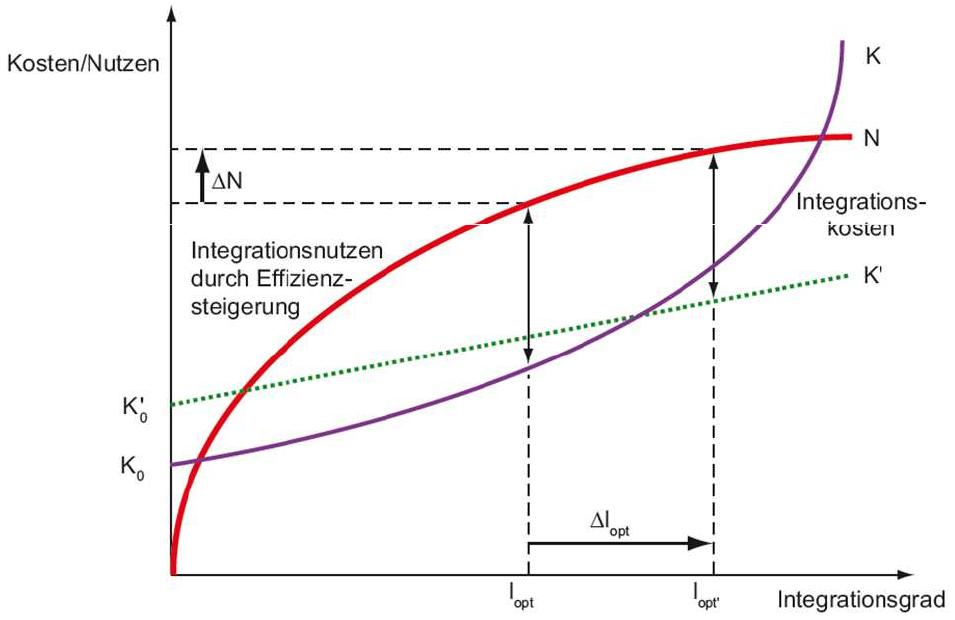
\includegraphics[width=0.75\textwidth]{img/V9.1.jpg}
			\caption{}
			\label{optIntegrGrad}
		\end{figure}
	\li Erklären Sie das Y-Integrationsmodell nach Scheer
	\li Was sind unternehmensweite Anwendungssysteme? Welche Aufgaben decken Sie ab?
	\li Erklären Sie, was ein Intranet von einem Exranet unterscheidet. Zählen Sie einige Eigenschaften und Vorteile eines Intranets auf.
	\li Nennen Sie in den Bereichen Finanz- und Rechnungswesen, Personalwesen, Produktion und Vertrieb/Marketing jeweils einige Funktionale Anwendungen eines Intranets.
	\li Was ist ein ERP-System? Welche Aufgaben deckt ein ERP System ab?
	\li Was unterscheidet die traditionelle Anordnung von Anwendungssystemen gegenüber einer Anordnung mit ERP-System?
	\li Nennen Sie einige Vor- und Nachteile/Herausforderungen eines ERP Systems.
	\li Was bedeutet Enterprise Application Integration EAI?
	\li Wie kann ein EAI die Komplexität verringern?
\olS




\end{document}
